\documentclass[aspectratio=169,11pt]{beamer}

% Presentación de Seminario de Título basada en main.tex
\usepackage[utf8]{inputenc}
\usepackage[T1]{fontenc}
% Babel en español cuando está instalado; fallback para TeX Live sin spanish.ldf.
\IfFileExists{spanish.ldf}{%
  \usepackage[spanish,es-noshorthands]{babel}%
  \spanishdecimal{.}%
}{%
  \usepackage[english]{babel}%
}
\usepackage{lmodern}
\usepackage{microtype}
\usepackage{amsmath,amssymb}
\usepackage{booktabs,tabularx,array,colortbl}
\usepackage{graphicx}
\usepackage{xcolor}
\usepackage{tikz}
\usetikzlibrary{shapes,arrows,arrows.meta,positioning,calc,fit,patterns,backgrounds,decorations.pathreplacing}
\usepackage{pgfplots}
\pgfplotsset{compat=1.15}
\usepackage{csquotes}
\usepackage[
  backend=biber,
  style=authoryear-comp,
  maxcitenames=2,
  maxbibnames=8,
  giveninits=true,
  uniquename=init,
  doi=false,
  url=false,
  isbn=false
]{biblatex}
\addbibresource{referencias.bib}

% Estilo visual tomado de ejemplojessica.tex
\definecolor{primary}{RGB}{15,76,110}
\definecolor{accent}{RGB}{224,122,40}
\definecolor{best}{RGB}{0,128,64}
\definecolor{warn}{RGB}{183,65,14}
\definecolor{inkgray}{RGB}{55,55,60}
\definecolor{lightbg}{RGB}{236,242,246}

% Alias para mantener editables los diagramas y tablas existentes
\colorlet{PUCVBlue}{primary}
\colorlet{PUCVBlueDark}{primary}
\colorlet{PUCVLight}{lightbg}
\colorlet{PUCVRed}{warn}
\colorlet{GreenH}{best}
\colorlet{WarmGold}{accent}
\colorlet{Ink}{inkgray}
\colorlet{Muted}{inkgray!78}
\colorlet{PaleGray}{lightbg}

\usetheme{default}
\useinnertheme{circles}
\setbeamercolor{normal text}{fg=inkgray}
\setbeamercolor{structure}{fg=primary}
\setbeamercolor{title}{fg=primary}
\setbeamercolor{subtitle}{fg=inkgray}
\setbeamercolor{frametitle}{fg=white,bg=primary}
\setbeamercolor{block title}{fg=white,bg=primary}
\setbeamercolor{block body}{fg=inkgray,bg=lightbg}
\setbeamercolor{block title alerted}{fg=white,bg=warn}
\setbeamercolor{block body alerted}{fg=inkgray,bg=warn!8}
\setbeamercolor{block title example}{fg=white,bg=best}
\setbeamercolor{block body example}{fg=inkgray,bg=best!8}
\setbeamercolor{itemize item}{fg=accent}
\setbeamercolor{itemize subitem}{fg=accent}
\setbeamercolor{section in toc}{fg=primary}
\setbeamercolor{author in head/foot}{fg=white,bg=primary!85}
\setbeamercolor{bibliography entry author}{fg=inkgray}
\setbeamercolor{bibliography entry title}{fg=inkgray!78}
\setbeamercolor{bibliography entry location}{fg=inkgray!78}
\setbeamercolor{bibliography entry note}{fg=inkgray!78}

\setbeamerfont{title}{series=\bfseries,size=\LARGE}
\setbeamerfont{subtitle}{size=\normalsize}
\setbeamerfont{frametitle}{series=\bfseries,size=\large}
\setbeamerfont{footline}{size=\scriptsize}

\setbeamertemplate{blocks}[rounded][shadow=false]
\setbeamertemplate{navigation symbols}{}
\setbeamertemplate{itemize items}[circle]
\setbeamertemplate{bibliography item}{\raisebox{0.2ex}{\tiny$\blacksquare$}}

% Banda superior y pie, iguales al estilo del ejemplo
\setbeamertemplate{frametitle}{%
  \nointerlineskip
  \begin{beamercolorbox}[wd=\paperwidth,ht=3.0ex,dp=1.2ex,leftskip=0.35cm,rightskip=0.35cm]{frametitle}%
    \usebeamerfont{frametitle}\insertframetitle%
  \end{beamercolorbox}%
}

\setbeamertemplate{footline}{%
  \leavevmode%
  \hbox{%
    \begin{beamercolorbox}[wd=.72\paperwidth,ht=2.4ex,dp=1.1ex,leftskip=0.35cm]{author in head/foot}%
      \usebeamerfont{footline}Series temporales y DTW/DDTW%
    \end{beamercolorbox}%
    \begin{beamercolorbox}[wd=.28\paperwidth,ht=2.4ex,dp=1.1ex,rightskip=0.35cm]{author in head/foot}%
      \usebeamerfont{footline}\hfill\insertframenumber\,/\,\inserttotalframenumber%
    \end{beamercolorbox}%
  }%
}

\newcommand{\smallcite}[1]{{\scriptsize\color{inkgray!72}\parencite{#1}}}
\newcommand{\key}[1]{\textcolor{primary}{\textbf{#1}}}
\newcommand{\risk}[1]{\textcolor{warn}{\textbf{#1}}}
\newcommand{\good}[1]{\textcolor{best}{\textbf{#1}}}
\newcommand{\destacado}[1]{\textcolor{primary}{\textbf{#1}}}
\newcommand{\gcell}{\cellcolor{primary!78}\color{white}\bfseries X}
\newcommand{\hcell}{\cellcolor{accent!24}\color{accent!70!black}\bfseries $\star$}

% Estilos de los diagramas (curvas ilustrativas, no resultados experimentales)
\pgfplotsset{
  convaxis/.style={
    axis lines=left,
    axis line style={inkgray!80},
    xtick=\empty, ytick=\empty,
    xmin=0, xmax=100, ymin=0,
    xlabel={Iteración}, ylabel={Mejor resultado encontrado},
    label style={font=\scriptsize, text=inkgray},
    xlabel style={yshift=2pt},
    ylabel style={yshift=-4pt},
    clip=false,
  },
  miniaxis/.style={
    convaxis,
    width=4.4cm, height=3.6cm,
    title style={font=\scriptsize\bfseries, text=inkgray, yshift=-4pt},
    ylabel={Mejor resultado},
  },
}
\tikzset{
  flujo/.style={draw=primary, fill=lightbg, rounded corners=3pt, thick,
    align=center, font=\footnotesize, text=inkgray, minimum height=1.0cm},
  flecha/.style={-{Stealth[length=5pt]}, thick, inkgray!80},
  llave/.style={decorate, decoration={brace, amplitude=4pt}, thick},
}


\title[Series temporales y DTW]{Coordinación de metaheurísticas colaborativas guiada por series temporales mediante Dynamic Time Warping}
\author{Lucas Erazo}
\institute{Escuela de Ingeniería Informática\ Pontificia Universidad Católica de Valparaíso}
\date{}

\begin{document}

\begin{frame}[plain]
  \nointerlineskip
  \makebox[\textwidth][s]{\hspace{0.1cm}
    
\includegraphics[width=7.0cm]{fig/logo_100.png}\hfill
    
\includegraphics[height=1.7cm]{fig/Logo_pucv_ok.PNG}\hspace{0.1cm}}
  \vspace{0.25cm}
  \titlepage
\end{frame}

\begin{frame}{Optimizar es elegir la mejor opción posible}
  \begin{columns}[c,onlytextwidth]
    \column{0.46\textwidth}
      \small
      Hay muchas opciones. Cada una obtiene un resultado, y algunas no son válidas porque se pasan de un límite.

      \vspace{0.35cm}
      \begin{block}{Qué se busca}
        La opción válida con el mejor resultado. No cualquiera que parezca buena.
      \end{block}
    \column{0.50\textwidth}
      \centering
      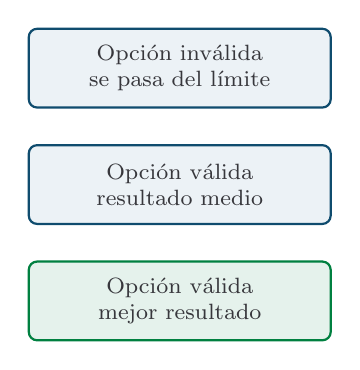
\begin{tikzpicture}
        \node[flujo, text width=3.6cm] (mala) {Opción inválida\\se pasa del límite};
        \node[flujo, text width=3.6cm, below=0.45cm of mala] (regular) {Opción válida\\resultado medio};
        \node[flujo, draw=best, fill=best!10, text width=3.6cm, below=0.45cm of regular] (mejor) {Opción válida\\mejor resultado};
      \end{tikzpicture}
  \end{columns}
\end{frame}

\begin{frame}{Revisar todas las opciones no alcanza}
  \begin{columns}[c,onlytextwidth]
    \column{0.48\textwidth}
      \small
      Si cada decisión es sí o no, veinte decisiones ya dan más de un millón de combinaciones.

      \vspace{0.3cm}
      En un problema real hay muchas más, y el tiempo para decidir es limitado.
    \column{0.48\textwidth}
      \centering
      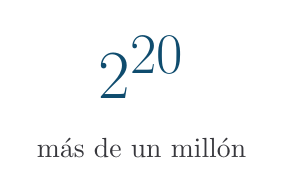
\begin{tikzpicture}
        \node[font=\Huge\bfseries, text=primary] (combinaciones) {$2^{20}$};
        \node[font=\normalsize, text=inkgray, below=0.25cm of combinaciones] {más de un millón};
      \end{tikzpicture}

      \vspace{0.45cm}
      \begin{exampleblock}{Consecuencia}
        Hay que buscar entre algunas, no enumerarlas todas.
      \end{exampleblock}
  \end{columns}
\end{frame}

\begin{frame}{Una metaheurística es una estrategia de búsqueda}
  \begin{columns}[c,onlytextwidth]
    \column{0.42\textwidth}
      \small
      Usa reglas generales para proponer opciones, evaluarlas y quedarse con la mejor hallada.

      \vspace{0.3cm}
      \begin{block}{Espacio de búsqueda}
        Es el conjunto de soluciones que podemos explorar.

        \medskip
        \key{Óptimo local:} ninguna solución vecina válida es mejor.

        \medskip
        \key{Óptimo global:} ninguna solución válida de todo el espacio es mejor.
      \end{block}
      {\footnotesize La metaheurística busca buenas soluciones, sin garantizar el óptimo global.}
    \column{0.54\textwidth}
      \centering
      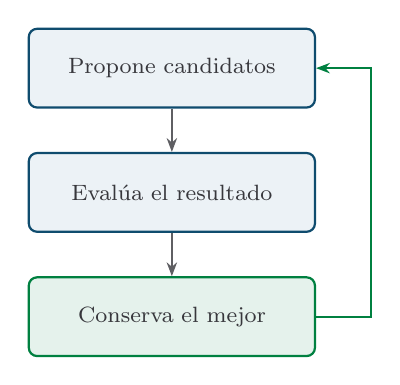
\begin{tikzpicture}[node distance=0.55cm]
        \node[flujo, text width=3.4cm] (propone) {Propone candidatos};
        \node[flujo, text width=3.4cm, below=of propone] (evalua) {Evalúa el resultado};
        \node[flujo, text width=3.4cm, draw=best, fill=best!10, below=of evalua] (guarda) {Conserva el mejor};
        \draw[flecha] (propone) -- (evalua);
        \draw[flecha] (evalua) -- (guarda);
        \draw[flecha, best] (guarda.east) -- ++(0.7,0) |- (propone.east);
      \end{tikzpicture}
  \end{columns}
\end{frame}

\begin{frame}{Equilibrar exploración y explotación}
  \begin{columns}[c,onlytextwidth]
    \column{0.48\textwidth}
      \begin{block}{Exploración}
        Busca en regiones distintas del espacio de búsqueda.
      \end{block}
      \centering
      \vspace{0.25cm}
      \begin{tikzpicture}
        \foreach \x/\y in {0.2/0.3, 1.5/1.6, 2.4/0.4, 3.6/1.8, 4.8/0.6, 5.6/1.4} {
          \fill[primary] (\x,\y) circle (2.5pt);
        }
      \end{tikzpicture}
    \column{0.48\textwidth}
      \begin{exampleblock}{Explotación}
        Aprovecha una región prometedora para mejorar las soluciones.
      \end{exampleblock}
      \centering
      \vspace{0.25cm}
      
\begin{tikzpicture}
        \foreach \x/\y in {2.2/1.0, 2.7/1.35, 3.1/0.95, 3.5/1.4, 3.9/1.15} {
          \fill[accent] (\x,\y) circle (2.5pt);
        }
        \fill[best] (3.15,1.2) circle (3.2pt);
      \end{tikzpicture}
  \end{columns}
  \vfill
  \centering
  \small Pueden alternarse durante la búsqueda: no son dos etapas fijas.
\end{frame}

\begin{frame}{El algoritmo útil cambia durante la búsqueda}
  \small
  Cada metaheurística combina exploración y explotación de manera distinta. El equilibrio adecuado puede cambiar durante la búsqueda.

  \vspace{0.35cm}
  \begin{tabularx}{\textwidth}{>{\bfseries\color{primary}}p{3.2cm} X}
    Al inicio & La exploración permite identificar regiones prometedoras. \\
    Durante la búsqueda & La explotación mejora soluciones en regiones prometedoras, sin abandonar la exploración. \\
    Al estancarse & Puede convenir cambiar de algoritmo y conservar lo ya encontrado. \\
  \end{tabularx}
\end{frame}

% Diagrama 1: curva de convergencia con progreso y estancamiento
\begin{frame}{Problema}
  \begin{block}{Pregunta}
    Durante la búsqueda, ¿cómo detectar que el proceso deja de mejorar y decidir qué hacer?
  \end{block}
  \vspace{0.1cm}
  \begin{columns}[c,onlytextwidth]
    \column{0.34\textwidth}
      \small
      La curva de convergencia muestra la evolución del mejor resultado encontrado.

      \vspace{0.35cm}
      Normalmente se revisa al final. Aquí se usa mientras la búsqueda todavía está en curso.
    \column{0.64\textwidth}
      \centering
      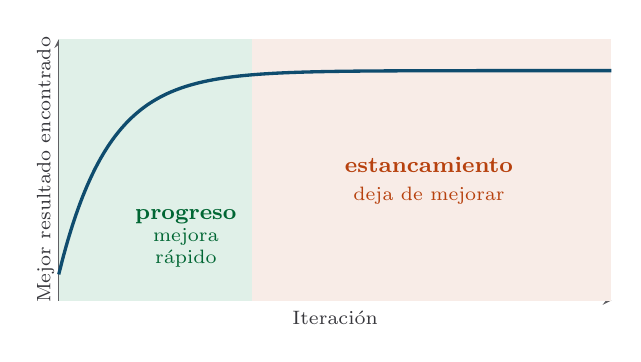
\begin{tikzpicture}
        \begin{axis}[convaxis, width=8.6cm, height=4.9cm, ymax=100]
          \fill[best!12] (0,0) rectangle (35,100);
          \fill[warn!10] (35,0) rectangle (100,100);
          \addplot[primary, very thick, domain=0:100, samples=120, smooth]
            {10 + 78*(1 - exp(-x/9))};
          \node[font=\footnotesize\bfseries, text=best!80!black] at (23,32) {progreso};
          \node[font=\scriptsize, text=best!80!black, align=center] at (23,20) {mejora\\rápido};
          \node[font=\footnotesize\bfseries, text=warn] at (67,52) {estancamiento};
          \node[font=\scriptsize, text=warn] at (67,40) {deja de mejorar};
        \end{axis}
      \end{tikzpicture}
  \end{columns}
\end{frame}

% Mismo contador, dos situaciones distintas
\begin{frame}{Contar iteraciones no alcanza}
  \begin{columns}[c,onlytextwidth]
    \column{0.42\textwidth}
      \small
      \begin{itemize}
        \item Un contador solo mide cuánto tiempo pasó sin una mejora.
        \item No describe si el avance es constante, lento o irregular.
        \item Un límite fijo puede depender del problema y del algoritmo.
      \end{itemize}
      \vspace{0.25cm}
      \begin{exampleblock}{Qué se necesita}
        Observar la forma reciente de la curva, no solo el tiempo transcurrido.
      \end{exampleblock}
    \column{0.56\textwidth}
      \centering
      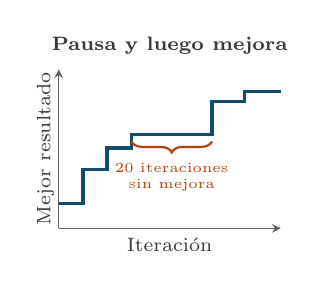
\begin{tikzpicture}
        \begin{axis}[miniaxis, xmax=55, ymax=95, title={Pausa y luego mejora}]
          \addplot[const plot, primary, very thick]
            coordinates {(0,15) (6,35) (12,48) (18,56) (38,76) (46,82) (55,82)};
          \draw[llave, warn, decoration={mirror}] (18,52) -- (38,52)
            node[midway, below=4pt, font=\tiny, text=warn, align=center] {20 iteraciones\\sin mejora};
        \end{axis}
      \end{tikzpicture}\hfill
      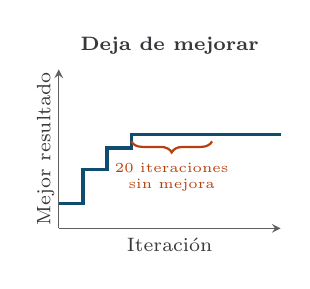
\begin{tikzpicture}
        \begin{axis}[miniaxis, xmax=55, ymax=95, title={Deja de mejorar}]
          \addplot[const plot, primary, very thick]
            coordinates {(0,15) (6,35) (12,48) (18,56) (55,56)};
          \draw[llave, warn, decoration={mirror}] (18,52) -- (38,52)
            node[midway, below=4pt, font=\tiny, text=warn, align=center] {20 iteraciones\\sin mejora};
        \end{axis}
      \end{tikzpicture}

      \vspace{0.15cm}
      {\footnotesize\risk{El contador ve lo mismo en ambos casos.}}
  \end{columns}
\end{frame}

% Diagrama 2: ventana reciente sobre la curva
\begin{frame}{La curva como serie temporal}
  \begin{columns}[c,onlytextwidth]
    \column{0.36\textwidth}
      \small
      Se toma una ventana reciente del mejor resultado.

      \vspace{0.3cm}
      Esa ventana es una \key{serie temporal}: una secuencia ordenada de valores.

      \vspace{0.3cm}
      \begin{block}{Dos situaciones}
        \begin{itemize}
          \item Sigue mejorando.
          \item Deja de mejorar.
        \end{itemize}
      \end{block}
    \column{0.62\textwidth}
      \centering
      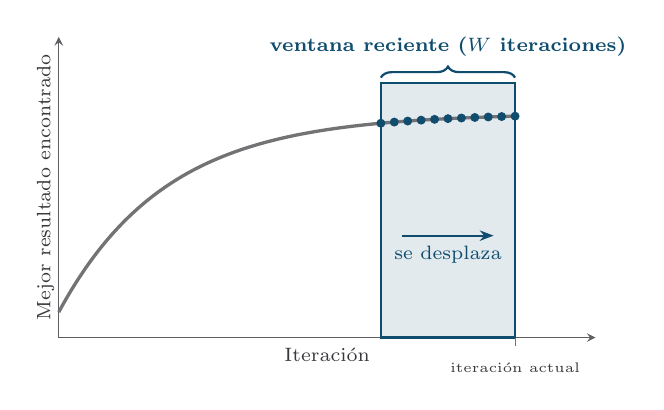
\begin{tikzpicture}
        \begin{axis}[convaxis, width=8.4cm, height=5.4cm, ymax=118]
          \fill[primary!12] (60,0) rectangle (85,100);
          \draw[primary, thick] (60,0) rectangle (85,100);
          \addplot[inkgray!70, very thick, domain=0:85, samples=100, smooth]
            {10 + 78*(1 - exp(-x/20))};
          \addplot[primary, only marks, mark=*, mark size=1.4pt, domain=60:85, samples=11]
            {10 + 78*(1 - exp(-x/20))};
          \draw[llave, primary] (60,102) -- (85,102)
            node[midway, above=4pt, font=\scriptsize\bfseries, text=primary]
            {ventana reciente ($W$ iteraciones)};
          \draw[flecha, primary] (64,40) -- (81,40)
            node[midway, below, font=\scriptsize, text=primary] {se desplaza};
          \draw[dashed, inkgray!70] (85,0) -- (85,-6)
            node[below, font=\tiny, text=inkgray] {iteración actual};
        \end{axis}
      \end{tikzpicture}
  \end{columns}
\end{frame}

% Diagrama 3: patrones de referencia
\begin{frame}{Dos patrones de comparación}
  \begin{columns}[T,onlytextwidth]
    \column{0.48\textwidth}
      \begin{exampleblock}{Progreso}
        El mejor resultado continúa mejorando dentro de la ventana.
      \end{exampleblock}
      \centering
      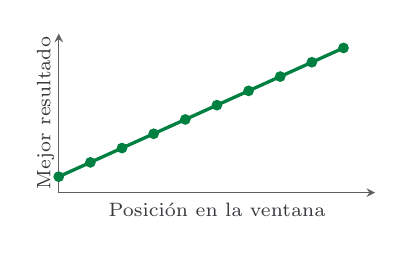
\begin{tikzpicture}
        \begin{axis}[convaxis, width=5.6cm, height=3.6cm, xmax=10, ymax=10,
                     xlabel={Posición en la ventana}, ylabel={Mejor resultado}]
          \addplot[best, very thick, mark=*, mark size=1.3pt, domain=0:9, samples=10] {1 + 0.9*x};
        \end{axis}
      \end{tikzpicture}
    \column{0.48\textwidth}
      \begin{alertblock}{Estancamiento}
        El mejor resultado se mantiene prácticamente igual.
      \end{alertblock}
      \centering
      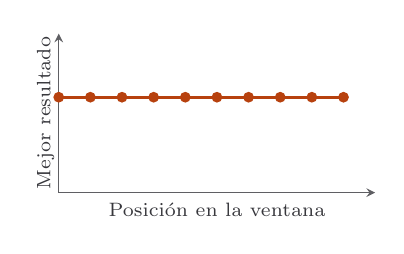
\begin{tikzpicture}
        \begin{axis}[convaxis, width=5.6cm, height=3.6cm, xmax=10, ymax=10,
                     xlabel={Posición en la ventana}, ylabel={Mejor resultado}]
          \addplot[warn, very thick, mark=*, mark size=1.3pt, domain=0:9, samples=10] {6};
        \end{axis}
      \end{tikzpicture}
  \end{columns}
  \vfill
  \centering
  \small No son ejemplos aprendidos: son patrones definidos para interpretar la curva.
\end{frame}

% Esquema didáctico: fig/make_convergence_mkp.py genera la figura
\begin{frame}{Una ventana, dos patrones de comparación}
  \centering
  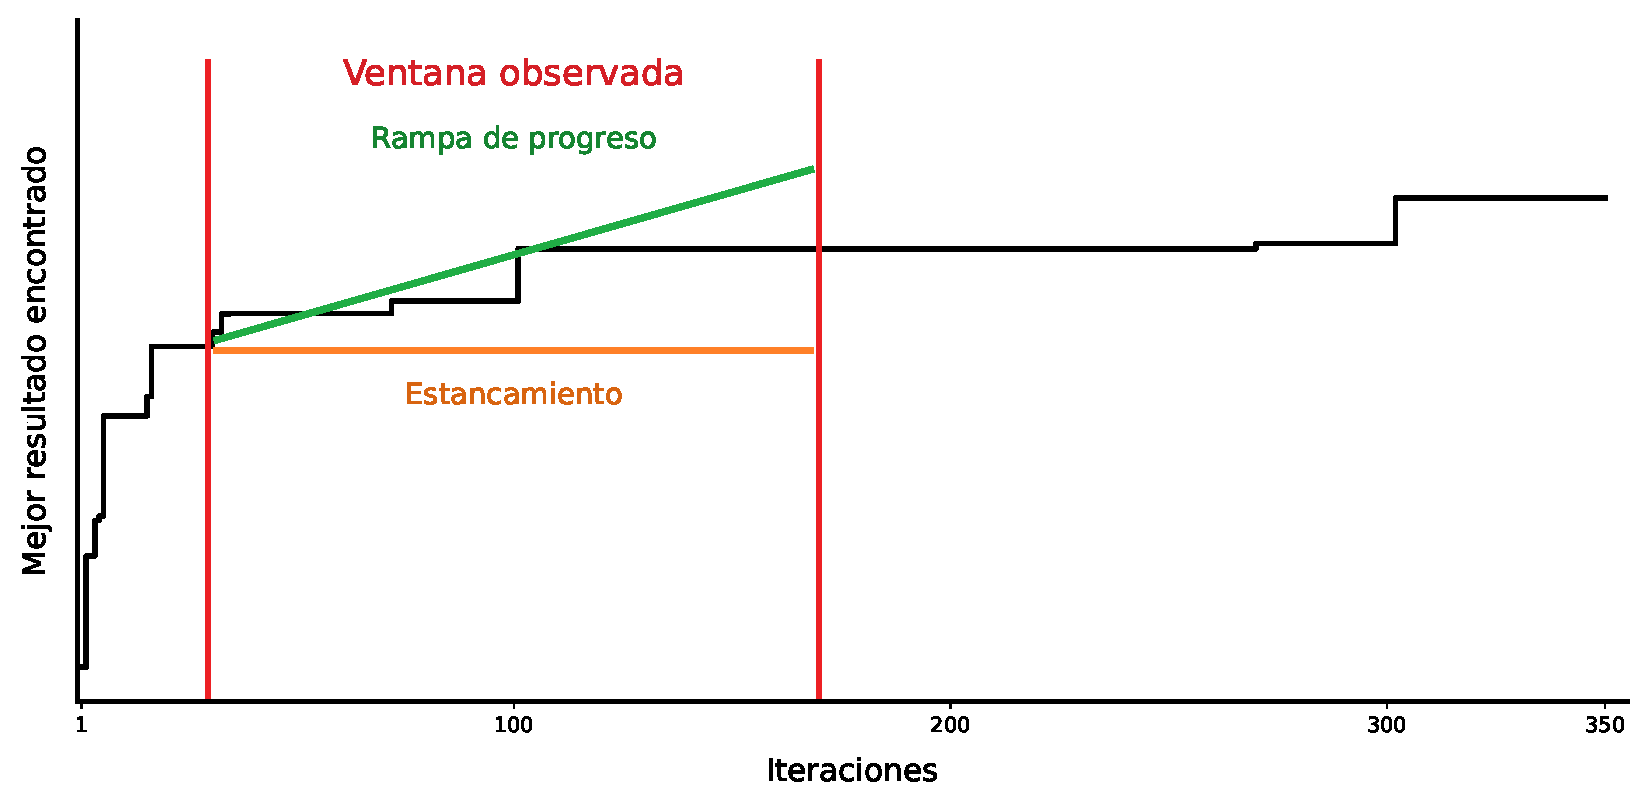
\includegraphics[width=0.96\textwidth,height=0.78\textheight,keepaspectratio]{fig/convergencia_mkp.pdf}
\end{frame}

% Diagrama 4: comparación rígida frente a alineamiento DTW
\begin{frame}{DTW y DDTW en simple}
  \small
  \begin{itemize}
    \item Comparan la forma de la ventana con los dos patrones.
    \item Reconocen formas parecidas aunque los cambios no ocurran al mismo tiempo.
  \end{itemize}
  \vspace{0.1cm}
  \centering
  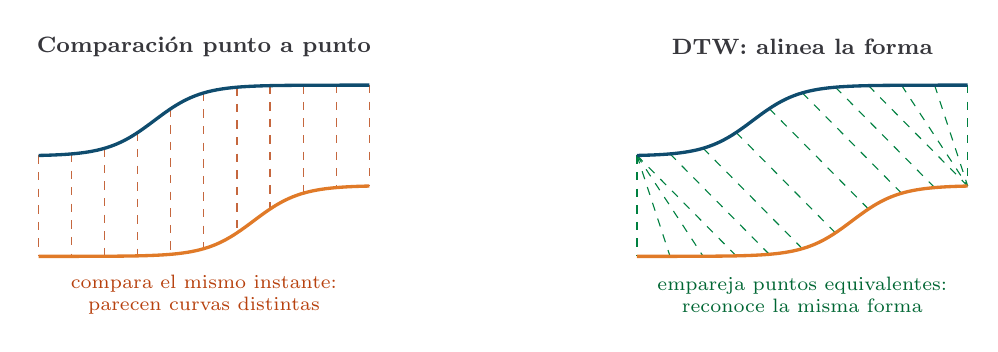
\begin{tikzpicture}[x=0.42cm, y=0.75cm]
    % Panel izquierdo: punto a punto
    \begin{scope}
      \node[font=\footnotesize\bfseries, text=inkgray] at (5,3.55) {Comparación punto a punto};
      \foreach \t in {0,...,10} {
        \pgfmathsetmacro{\ya}{1.7 + 1.2/(1 + exp(-1.4*(\t - 3.5)))}
        \pgfmathsetmacro{\yb}{0.0 + 1.2/(1 + exp(-1.4*(\t - 6.5)))}
        \draw[dashed, warn!80] (\t,\ya) -- (\t,\yb);
      }
      \draw[primary, very thick, smooth, samples=40, domain=0:10]
        plot (\x, {1.7 + 1.2/(1 + exp(-1.4*(\x - 3.5)))});
      \draw[accent, very thick, smooth, samples=40, domain=0:10]
        plot (\x, {0.0 + 1.2/(1 + exp(-1.4*(\x - 6.5)))});
      \node[font=\scriptsize, text=warn, align=center] at (5,-0.65)
        {compara el mismo instante:\\parecen curvas distintas};
    \end{scope}
    % Panel derecho: DTW
    \begin{scope}[xshift=7.6cm]
      \node[font=\footnotesize\bfseries, text=inkgray] at (5,3.55) {DTW: alinea la forma};
      \foreach \i/\j in {0/0,0/1,0/2,0/3,1/4,2/5,3/6,4/7,5/8,6/9,7/10,8/10,9/10,10/10} {
        \pgfmathsetmacro{\ya}{1.7 + 1.2/(1 + exp(-1.4*(\i - 3.5)))}
        \pgfmathsetmacro{\yb}{0.0 + 1.2/(1 + exp(-1.4*(\j - 6.5)))}
        \draw[dashed, best] (\i,\ya) -- (\j,\yb);
      }
      \draw[primary, very thick, smooth, samples=40, domain=0:10]
        plot (\x, {1.7 + 1.2/(1 + exp(-1.4*(\x - 3.5)))});
      \draw[accent, very thick, smooth, samples=40, domain=0:10]
        plot (\x, {0.0 + 1.2/(1 + exp(-1.4*(\x - 6.5)))});
      \node[font=\scriptsize, text=best!80!black, align=center] at (5,-0.65)
        {empareja puntos equivalentes:\\reconoce la misma forma};
    \end{scope}
  \end{tikzpicture}

  \vspace{0.15cm}
  \begin{tabularx}{\textwidth}{p{2.2cm} X}
    \key{DTW} & Compara los valores de las curvas. \\
    \key{DDTW} & Compara cómo cambian esas curvas. \\
  \end{tabularx}
\end{frame}

% Diagrama 4b: DDTW mira los cambios entre iteraciones
\begin{frame}{DDTW: comparar los cambios}
  \begin{columns}[c,onlytextwidth]
    \column{0.36\textwidth}
      \small
      DTW compara los \key{valores} de la curva.

      \vspace{0.3cm}
      DDTW compara \key{cuánto cambia} la curva de un paso al siguiente.

      \vspace{0.3cm}
      \begin{block}{Lectura}
        Si los cambios se acercan a cero, la búsqueda dejó de mejorar.
      \end{block}
    \column{0.62\textwidth}
      \centering
      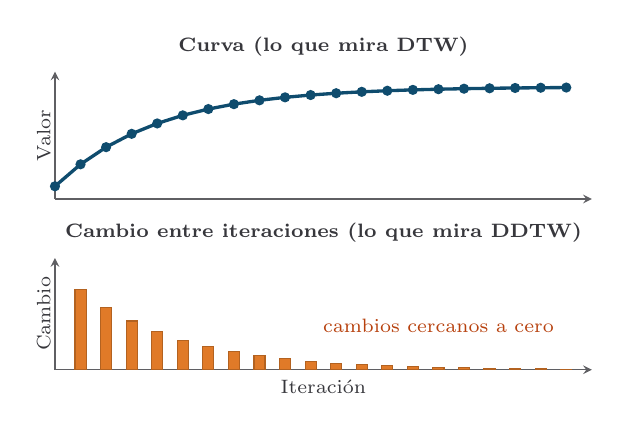
\begin{tikzpicture}
        \begin{axis}[convaxis, name=valor, width=8.4cm, height=3.2cm,
                     xmin=0, xmax=21, ymax=100, xlabel={}, ylabel={Valor},
                     title={Curva (lo que mira DTW)},
                     title style={font=\scriptsize\bfseries, text=inkgray, yshift=-4pt}]
          \addplot[primary, very thick, mark=*, mark size=1.2pt, domain=0:20, samples=21]
            {10 + 78*(1 - exp(-x/4))};
        \end{axis}
        \begin{axis}[convaxis, at={(valor.south west)}, anchor=north west, yshift=-0.75cm,
                     width=8.4cm, height=3.0cm,
                     xmin=0, xmax=21, ymax=24, ylabel={Cambio},
                     title={Cambio entre iteraciones (lo que mira DDTW)},
                     title style={font=\scriptsize\bfseries, text=inkgray, yshift=-4pt}]
          \addplot[ybar, bar width=4pt, fill=accent, draw=accent!80!black, domain=1:20, samples=20]
            {78*(exp(-(x-1)/4) - exp(-x/4))};
          \node[font=\scriptsize, text=warn, anchor=south] at (15,6) {cambios cercanos a cero};
        \end{axis}
      \end{tikzpicture}
  \end{columns}
\end{frame}

% Diagrama 5: persistencia antes de cambiar
\begin{frame}{Cómo se confirma el estancamiento}
  \small
  \begin{enumerate}
    \item La ventana se parece al patrón de estancamiento.
    \item Se aleja del patrón de progreso.
    \item Esa condición se mantiene durante varias actualizaciones.
  \end{enumerate}
  \vspace{0.1cm}
  \centering
  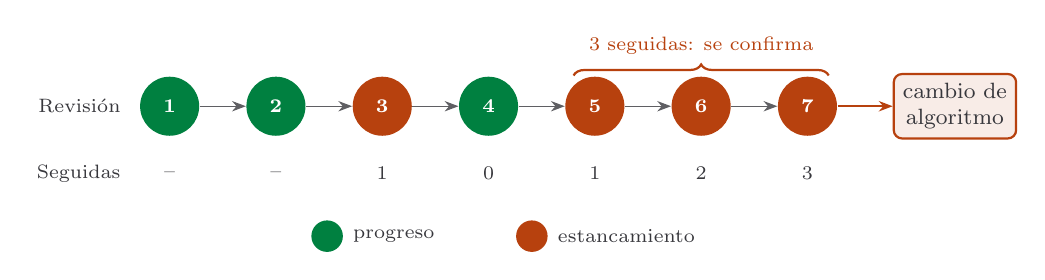
\begin{tikzpicture}[
      rev/.style={circle, minimum size=0.75cm, font=\scriptsize\bfseries, text=white, inner sep=0pt},
      prog/.style={rev, fill=best},
      est/.style={rev, fill=warn}]
    \node[font=\scriptsize, text=inkgray, anchor=east] at (-0.5,0) {Revisión};
    \node[font=\scriptsize, text=inkgray, anchor=east] at (-0.5,-0.85) {Seguidas};
    \foreach \k/\tipo/\c in {1/prog/--, 2/prog/--, 3/est/1, 4/prog/0, 5/est/1, 6/est/2, 7/est/3} {
      \node[\tipo] (r\k) at ({(\k-1)*1.35},0) {\k};
      \node[font=\scriptsize, text=inkgray] at ({(\k-1)*1.35},-0.85) {\c};
    }
    \foreach \a/\b in {1/2,2/3,3/4,4/5,5/6,6/7} { \draw[flecha, thin] (r\a) -- (r\b); }
    \node[flujo, draw=warn, fill=warn!10, minimum height=0.8cm, right=0.7cm of r7] (cambio) {cambio de\\algoritmo};
    \draw[flecha, warn] (r7) -- (cambio);
    \draw[llave, warn] ($(r5.north west)+(0,0.12)$) -- ($(r7.north east)+(0,0.12)$)
      node[midway, above=4pt, font=\scriptsize, text=warn] {3 seguidas: se confirma};
    \node[prog, minimum size=0.4cm, label={[font=\scriptsize, text=inkgray]right:progreso}] at (2.0,-1.65) {};
    \node[est, minimum size=0.4cm, label={[font=\scriptsize, text=inkgray]right:estancamiento}] at (4.6,-1.65) {};
  \end{tikzpicture}

  \vspace{0.05cm}
  \begin{block}{Para qué sirve la persistencia}
    Evita reaccionar ante una fluctuación aislada.
  \end{block}
\end{frame}

% Diagrama 6: respuesta con cambio de algoritmo sin perder el mejor
\begin{frame}{Qué hacer al detectarlo}
  \begin{columns}[c,onlytextwidth]
    \column{0.36\textwidth}
      \small
      \begin{block}{Respuesta}
        Cambiar el algoritmo activo, conservar el mejor resultado encontrado y continuar la búsqueda.
      \end{block}
      \vspace{0.2cm}
      \begin{itemize}
        \item No se reinicia el proceso.
        \item No se descarta lo encontrado.
        \item El momento del cambio depende de la curva observada.
      \end{itemize}
    \column{0.62\textwidth}
      \centering
      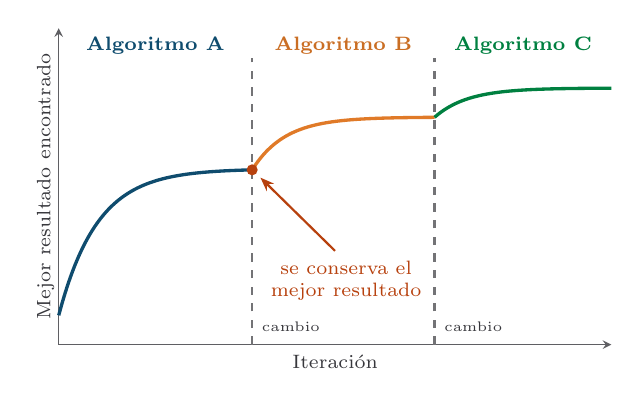
\begin{tikzpicture}
        \begin{axis}[convaxis, width=8.6cm, height=5.6cm, ymax=108]
          \addplot[primary, very thick, domain=0:35, samples=60, smooth]
            {10 + 50*(1 - exp(-x/7))};
          \addplot[accent, very thick, domain=35:68, samples=60, smooth]
            {10 + 50*(1 - exp(-35/7)) + 18*(1 - exp(-(x-35)/6))};
          \addplot[best, very thick, domain=68:100, samples=60, smooth]
            {10 + 50*(1 - exp(-35/7)) + 18*(1 - exp(-33/6)) + 10*(1 - exp(-(x-68)/6))};
          \draw[dashed, inkgray!70, thick] (35,0) -- (35,98);
          \draw[dashed, inkgray!70, thick] (68,0) -- (68,98);
          \node[font=\scriptsize\bfseries, text=primary] at (17.5,102) {Algoritmo A};
          \node[font=\scriptsize\bfseries, text=accent!90!black] at (51.5,102) {Algoritmo B};
          \node[font=\scriptsize\bfseries, text=best] at (84,102) {Algoritmo C};
          \node[font=\tiny, text=inkgray, anchor=west] at (35,6) {cambio};
          \node[font=\tiny, text=inkgray, anchor=west] at (68,6) {cambio};
          \fill[warn] (35,59.66) circle (2pt);
          \draw[flecha, warn] (50,32) -- (36.5,57);
          \node[font=\scriptsize, text=warn, align=center, anchor=north] at (52,32)
            {se conserva el\\mejor resultado};
        \end{axis}
      \end{tikzpicture}
  \end{columns}
\end{frame}

% Diagrama 7: flujo completo
\begin{frame}{El proceso completo}
  \centering
  \vspace{0.2cm}
  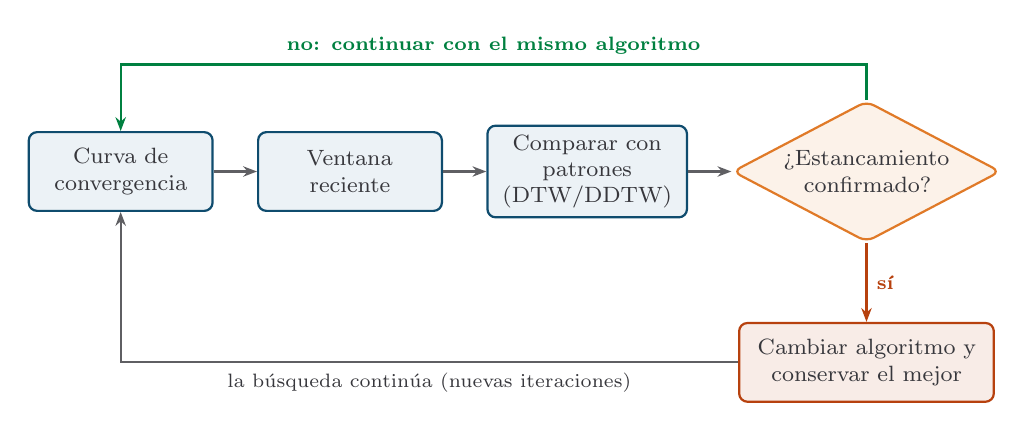
\begin{tikzpicture}[node distance=0.55cm]
    \node[flujo, text width=2.1cm] (curva) {Curva de\\convergencia};
    \node[flujo, text width=2.1cm, right=of curva] (ventana) {Ventana\\reciente};
    \node[flujo, text width=2.3cm, right=of ventana] (dtw) {Comparar con\\patrones\\(DTW/DDTW)};
    \node[flujo, diamond, aspect=1.9, inner sep=1pt, text width=2.2cm, draw=accent, fill=accent!10,
          right=of dtw] (dec) {¿Estancamiento\\confirmado?};
    \node[flujo, text width=3.0cm, draw=warn, fill=warn!10, below=1.0cm of dec] (cambiar)
      {Cambiar algoritmo y\\conservar el mejor};
    \draw[flecha] (curva) -- (ventana);
    \draw[flecha] (ventana) -- (dtw);
    \draw[flecha] (dtw) -- (dec);
    \draw[flecha, warn] (dec) -- node[right, font=\scriptsize\bfseries, text=warn] {sí} (cambiar);
    \draw[flecha, best] (dec.north) -- ++(0,0.45) -| node[pos=0.25, above, font=\scriptsize\bfseries, text=best]
      {no: continuar con el mismo algoritmo} (curva.north);
    \draw[flecha] (cambiar) -| node[pos=0.25, below, font=\scriptsize, text=inkgray]
      {la búsqueda continúa (nuevas iteraciones)} (curva.south);
  \end{tikzpicture}

  \vspace{0.35cm}
  \small La revisión se repite durante toda la búsqueda; nunca se reinicia desde cero.
\end{frame}

% Contraste: sin entrenamiento previo
\begin{frame}{Una ventaja importante}
  \begin{exampleblock}{No requiere entrenamiento}
    DTW compara la curva actual con dos patrones fijos. No necesita datos históricos ni una política aprendida.
  \end{exampleblock}
  \vspace{0.2cm}
  \centering
  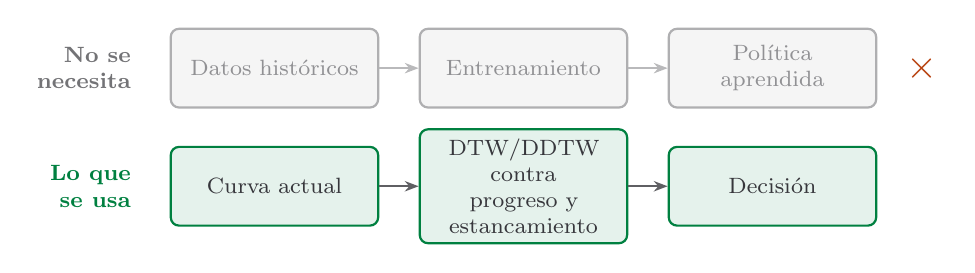
\begin{tikzpicture}[node distance=0.5cm]
    \node[font=\footnotesize\bfseries, text=inkgray!70, anchor=east, align=right] at (-0.3,0) {No se\\necesita};
    \node[flujo, text width=2.4cm, draw=inkgray!40, fill=inkgray!5, text=inkgray!55] (h1) at (1.4,0) {Datos históricos};
    \node[flujo, text width=2.4cm, draw=inkgray!40, fill=inkgray!5, text=inkgray!55, right=of h1] (h2) {Entrenamiento};
    \node[flujo, text width=2.4cm, draw=inkgray!40, fill=inkgray!5, text=inkgray!55, right=of h2] (h3) {Política\\aprendida};
    \draw[flecha, inkgray!35] (h1) -- (h2);
    \draw[flecha, inkgray!35] (h2) -- (h3);
    \node[font=\Large\bfseries, text=warn, right=0.25cm of h3] {$\times$};

    \node[font=\footnotesize\bfseries, text=best, anchor=east, align=right] at (-0.3,-1.5) {Lo que\\se usa};
    \node[flujo, text width=2.4cm, draw=best, fill=best!10] (u1) at (1.4,-1.5) {Curva actual};
    \node[flujo, text width=2.4cm, draw=best, fill=best!10, right=of u1] (u2) {DTW/DDTW contra\\progreso y estancamiento};
    \node[flujo, text width=2.4cm, draw=best, fill=best!10, right=of u2] (u3) {Decisión};
    \draw[flecha] (u1) -- (u2);
    \draw[flecha] (u2) -- (u3);
  \end{tikzpicture}

  \vspace{0.3cm}
  \small Esa comparación indica estancamiento durante la búsqueda. No es un uso habitual de DTW.
\end{frame}

\begin{frame}{Idea central}
  \begin{enumerate}
    \item La curva de convergencia se analiza durante la búsqueda.
    \item DTW o DDTW reconoce si su forma indica progreso o estancamiento.
    \item Al confirmar el estancamiento, se cambia de algoritmo sin perder el mejor resultado.
  \end{enumerate}
  \vfill
  \centering
  \key{La serie temporal informa la decisión; no sirve solo para el gráfico final.}
\end{frame}

\end{document}
